Relaciona con una l\'inea recta cada figura con la clasificación del par de ángulos (verde y azul) que se resaltan en ella.
\begin{center}
    \begin{minipage}{0.3\linewidth}
        \begin{parts}
            \part 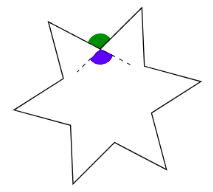
\includegraphics[height=2.5cm]{Images/poly_angle_01}
            \hfill{\color{cadmiumgreen}$\square$}
            \part 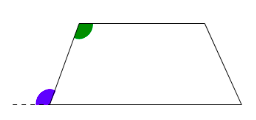
\includegraphics[height=1.8cm]{Images/poly_angle_02}
            \hfill{\color{cadmiumgreen}$\square$}
            \part 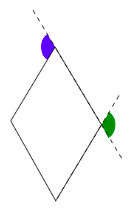
\includegraphics[height=3cm]{Images/poly_angle_03}
            \hfill{\color{cadmiumgreen}$\square$}
            \part 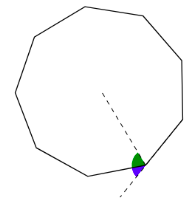
\includegraphics[height=2.5cm]{Images/poly_angle_04}
            \hfill{\color{cadmiumgreen}$\square$}
            \part 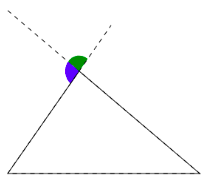
\includegraphics[height=2.8cm]{Images/poly_angle_05}
            \hfill{\color{cadmiumgreen}$\square$}
            \part 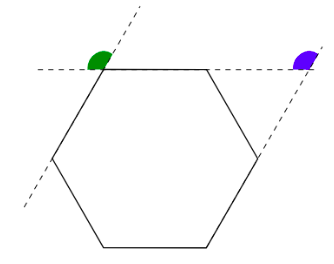
\includegraphics[height=2.8cm]{Images/poly_angle_06}
            \hfill{\color{cadmiumgreen}$\square$}
        \end{parts}
    \end{minipage}\hspace{1cm}
    \begin{minipage}{0.4\linewidth}
        \checkboxchar{ {\color{cadmiumorange}
                    $\Box$}
        }
        \begin{checkboxes}
            \choice Suplementarios                \vspace{2cm}
            \choice Correspondientes              \vspace{2cm}
            \choice Alternos externos             \vspace{2cm}
            \choice Adyacentes no suplementarios  \vspace{2cm}
            \choice Opuestos por el vértice       \vspace{2cm}
            \choice Alternos internos
        \end{checkboxes}
    \end{minipage}
\end{center}